\chapter{O ciclo de vida do produto na I4.0}
\label{cha:ciclo-de-vida}

Este capítulo traz detalhes da integração da memória digital do produto (MDP) ao Componente 4.0 (C4.0) para que assim possa ser compartilhado pelo cadeia de suprimentos.

Além disso, é abordada uma proposta de modelo de dados para os submodelos que compartilham informações relacionadas ao estado do produto na cadeia de suprimentos. Desta forma, é feita uma análise dos submodelos relevantes a serem compartilhados com os seus respectivos atributos.

Por fim, este capítulo traz discussões sobre o impacto do amplo compartilhamento da memória digital do produto (MDP) ao longo da cadeia de suprimentos por meio de serviços na Indústria 4.0. Uma visão da MDP sobre o eixo ``Ciclo de Vida e Cadeia de Valor'' é apresentada com considerações sobre a geração de valor por meio do compartilhamento da MDP ao longo ciclo de vida de um produto

% São abordadas possíveis mudanças na curva de ciclo de vida do produto e o surgimento de novos modelos de negócio baseado em dados (\textit{data-driven}).

%Uma visão da MDP sobre o eixo ``Ciclo de Vida e Cadeia de Valor'' do RAMI4.0 é abordada, discutindo como o compartilhamento de informações se relaciona com o ASS em sua forma ``tipo'' e ``instância''.

\section{Integração da MDP ao Componente 4.0}
\label{sec:estrutura-aas}

O conceito de Memória Digital do Produto (MDP) deve ser inserido na Indústria 4.0 com o objetivo de se agregar valor ao produto por meio da possibilidade de acesso a informações sobre o ativo entre parceiros ao longo da cadeia de suprimentos.

Nesta seção são apresentados os detalhes sobre uma possível estruturação do \textit{Asset Administration Shell} (AAS), que é parte de um Componente 4.0 (C4.0), contendo todas as partes necessárias (incluindo a MDP) para a implementação do compartilhamento de informações por meio de \textit{Web Services} (WS).

A estruturação proposta é baseada em \citeonline{bader2019aas}, que estabelece a divisão do AAS em submodelos.

% O cabeçalho na estrutura proposta terá a função de providenciar informações públicas sobre o ativo que o identifiquem minimamente e que forneça uma descrição sobre seus serviços oferecidos. O cabeçalho deverá conter informações que podem ser acessadas sem a necessidade de autenticação como, por exemplo, seu identificador único universal (UUID - \textit{Universal Unique IDentifier}), o modelo e fabricante do ativo. O cabeçalho deverá conter também o contrato daquele \textit{Web Service} com as descrições de seus serviços públicos disponíveis.

% O cabeçalho não terá a função de fornecer uma ficha técnica detalhada, mas apenas uma caracterização abstrata das funções/serviços do ativo. O cabeçalho deverá necessariamente conter o UUID do AAS. Sem o UUID o C4.0-Servidor se torna inacessível para qualquer uma das partes da cadeia de suprimentos.

% O corpo de um AAS fornece as informações e funcionalidades sensíveis sobre o ativo, que podem ser acessadas mediante autenticação.

As funcionalidades dos ativos são agrupadas em forma de submodelos, conforme estabelecido em \citeonline{bader2019aas, adolph2018roadmap, bedenbender2017aasexamples}, que são unidades de agrupamento de propriedades semelhantes. Os dados do ativo são armazenados nos próprios submodelos, enquanto a MDP extrai e gerencia as informações dos submodelos de forma a estruturá-las para serem diretamente fornecidas ao consumidor por meio de \textit{Web Services}.

A MDP no contexto de um C4.0 agrega as informações referentes a cada um dos submodelos e as organiza de forma a poderem ser facilmente disponibilizadas por meio de WSs.

Como a MDP é parte integral do AAS do C4.0, que representa a parte virtual do ativo, esta pode ser fornecida em qualquer meio digital, inclusive em armazenamentos remotos em plataformas na nuvem. Estas plataformas específicas suportam o armazenamento de grandes quantidades de dados, assim como podem assegurar uma alta capacidade de processamento de requisições de serviços.

A estrutura do C4.0 compatível com a arquitetura orientada a serviços proposta é apresentada na \autoref{fig:estrutura-aas}.

\begin{figure}[htb]
	\centering
	\includegraphics[width=0.7\textwidth]{estrutura-aas}
	\caption{Estrutura do Componente 4.0 com seus submodelos e a MDP.}
	\label{fig:estrutura-aas}
\end{figure}

Os dados puros estão contidos nos submodelos. A MDP fornece uma interface para a leitura e escrita dos dados dos submodelos. A MDP atua como um ponto único de extração de dados dos submodelos, evitando desta forma a extração de dados não tratados diretamente dos submodelos.

A MDP é capaz de realizar o gerenciamento dos dados, estabelecendo, por exemplo, políticas de acesso e/ou escrita e demais regras de negócio do produto. Uma analogia é de que os submodelos representam o banco de dados, enquanto a MDP é a interface para as operações de criação, leitura, atualização e exclusão (operações CRUD - \textit{Create, Read, Update, Delete}) nesta base de dados que são os submodelos.

Neste trabalho é dado foco aos submodelos que se relacionam a informações sobre o produto que sejam de interesse às partes ao longo da cadeia de suprimentos e que possam ser lidos ou escritos por meio dos WSs. Alguns exemplos desse tipo de submodelo podem incluir: a ficha técnica detalhada do ativo, submodelos de histórico de leitura de sensores, histórico de leitura de geolocalização (GPS), histórico de padrões de uso, etc. A relevância sobre cada uma dessas informações a serem armazenadas pela MDP e os impactos do amplo compartilhamento dessas informações ao longo da cadeia de suprimentos são discutidos na \autoref{sec:submodelos-produto}.

\section{Submodelos do produto}
\label{sec:submodelos-produto}

Nesta seção são apresentadas propostas de submodelos e atributos necessários para a integração dos ativos na cadeia de suprimentos. Os submodelos devem ser padronizados e detalhados a fim de garantir a interoperabilidade entre os sistemas.

O produto no contexto da ``Arquitetura para compartilhamento de informações do ativo'' é a fonte e o servidor de informações para os diversos membros ao longo da cadeia de suprimentos. O acesso a estas informações permite a colaboração entre os membros e assim abre oportunidades para uma tomada de decisões coordenada a fim de remover as ineficiências inerentes à cadeia de suprimentos.

É necessária uma definição dos submodelos do produto para que se possa identificar os tipos de informações a serem compartilhadas e com quais membros compartilhar. Além disso, a definição destes submodelos contribui com o refinamento das especificações do AAS no contexto da Indústria 4.0.

\citeonline{torres2014information} em uma análise de literatura mostra o impacto do compartilhamento de informações e de diferentes estratégias de colaboração no desempenho de cadeias de suprimentos. Além disso, é feita uma classificação dos trabalhos, dentre elas a classificação quanto ao tipo de informação a ser compartilhada, apresentando também a descrição de informações comumente mencionadas nos trabalhos.

Além disso, \citeonline{bader2020submodel} definem alguns tipos de submodelos padrões para a Indústria 4.0 e detalha seus respectivos atributos.

Os tipos de informações identificados na análise bibliográfica de \citeonline{torres2014information} e no documento de \citeonline{bader2020submodel} serão incorporados a novos submodelos propostos para o produto para que possam ser compartilhados por meio da MDP ao longo da cadeia de suprimentos.

Os submodelos propostos são baseados na classificação das informações contidas em cada submodelo. Os submodelos propostos são: ``Dados Gerais'', ``Processos'', ``Inventário'', ``Pedido'', ``Operação'' e ``Documentação''.

Além disso, os submodelos são classificados como ``família'', onde as informações estão relacionadas a um conjunto de instâncias de um produto de mesma família/classe, e também classificados como ``unitário'', onde a informação é relativa a uma instância específica de um produto unitário.

A \autoref{fig:submodelos-produto} mostra os submodelos propostos juntamente com sua classificação. Os mesmos submodelos são detalhados nas subseções seguintes.

\begin{figure}[htb!]
	\centering
	\includegraphics[width=1\textwidth]{submodelos-produto}
	\caption{Submodelos do C4.0-Servidor e seus atributos.}
	\label{fig:submodelos-produto}
\end{figure}

\newpage

%Portanto, são detalhados os seguintes submodelos referentes ao AAS-Produto: ``Processo'', ``Recursos'', ``Inventário'', ``Pedido'', ``Planejamento'', ``Dados técnicos'', ``Dados Operacionais'' e ``Documentação'' (Tabelas \ref{tab:produto-submodelo-processo}, \ref{tab:produto-submodelo-recursos}, \ref{tab:produto-submodelo-inventario}, \ref{tab:produto-submodelo-pedido}, \ref{tab:produto-submodelo-planejamento}).

%O objetivo de se especificar os submodelos de um AAS (contido em um C4.0) é o estabelecimento de um formato padrão de estrutura de dados, criando uma interface pela qual desenvolvedores, fabricantes e editores de documentação técnica possam se basear na hora de descrever os seus próprios produtos.

\subsection{Submodelo ``Dados Gerais''}

O AAS do C4.0-Servidor deve conter um submodelo que represente as informações gerais relacionadas ao produto que são de acesso público.

Este submodelo é baseado no template de submodelo ``\textit{Nameplate}'' (Placa de Identificação) introduzido por \citeonline{bader2020submodel}, que tem como alvo principal equipamentos para indústria de processos e automação industrial.

As informações neste submodelo descrevem como as características do produto estarão visíveis para os membros da cadeia de suprimentos.

Dentro deste modelo, todas as propriedades são comuns a uma família de produtos.

A \autoref{tab:submodelo-dados-gerais} detalha o submodelo ``Dados Gerais'' com seus respectivos atributos.

\begin{longtable}{p{.20\textwidth} p{.08\textwidth} p{.60\textwidth}}
	\caption{Atributos do submodelo ``Dados Gerais''.
	}                                                                                                                                                                            \\


	\hline
	\textbf{Propriedade}
	 & \textbf{Tipo}
	 & \textbf{Descrição}                                                                                                                                                        \\

	\hline
	Nome do produto
	 & \makecell{String}
	 & Título que constitui a denominação comercial do objeto/produto.
	\\

	\hline
	Código do produto
	 & \makecell{String}
	 & Conjunto de números e/ou letras para identificação do modelo do produto.
	\\

	\hline
	Imagem do produto
	 & \makecell{MIME\\{image/jpg}}
	 & Arquivo de imagem do produto em um formato de imagem comum \cite{bader2020submodel}.
	\\

	\hline
	Nome do fabricante
	 & \makecell{String}
	 & Designação legalmente válida do órgão natural ou judicial diretamente responsável pela concepção, produção, embalagem e rotulagem de um produto \cite{bader2020submodel}.
	\\

	\hline
	Logo do fabricante
	 & \makecell{MIME\\{image/jpg}}
	 & Arquivo de imagem da logo do fabricante em um formato de imagem comum \cite{bader2020submodel}.
	\\

	\hline
	\label{tab:submodelo-dados-gerais}
\end{longtable}

\subsection{Submodelo ``Processos''}

O submodelo ``Processos'' do AAS do C4.0-Servidor descreve informações relacionadas a processos de negócio aplicados ao produto a fim de satisfazer as demandas do cliente, isto é, as etapas de pedido, produção e envio.

A etapa de pedido começa quando um comprador faz um pedido ao fornecedor e termina quando o fornecedor aceita o pedido. A etapa de produção ocorre com a transformação dos materiais de entrada em um produto de maior valor. A etapa de envio entrega as mercadorias do fornecedor ao comprador. Diferentes tipos de informações estão relacionados a cada uma destas etapas.

Todas as propriedades desde submodelo se referem a uma família de produtos.

A \autoref{tab:submodelo-processos} detalha o submodelo ``Processos'' com seus respectivos atributos.

\begin{longtable}{p{.20\textwidth} p{.08\textwidth} p{.60\textwidth}}
	% \centering
	\caption{Atributos do submodelo ``Processos''.}                                                                                                                                                                                                                                                                                                                                                                                                                                                                                                                                                                                                                   \\

	% \begin{tabular}{p{3.5cm}p{1.5cm}p{9cm}}
	\hline
	\textbf{Propriedade}
	 & \textbf{Tipo}
	 & \textbf{Descrição}                                                                                                                                                                                                                                                                                                                                                                                                                                                                                                                                                                                                                                             \\



	\hline
	Tipo de processo fabricação
	 & \textit{Double}
	 & Tipo de processo de fabricação utilizado. Dado que diferentes empresas podem produzir um produto utilizando processos de fabricação distintos, este atributo permite que o cliente possa selecionar/filtrar um fornecedor com base no processo desejado. Além disso, este atributo é utilizado para equiparar fornecedores que utilizam um mesmo processo de fabricação, não prejudicando assim um fornecedor que usa um processo mais caro, porém mais moderno.                                                                                                                                                                                               \\

	\hline
	Custo do processo de fabricação
	 & \textit{Double}
	 & Custo total do processo de fabricação. O compartilhamento dos custos do processo é necessário no planejamento integrado da cadeia de suprimentos.                                                                                                                                                                                                                                                                                                                                                                                                                                                                                                              \\
	\hline
	Qualidade do processo de fabricação
	 & \textit{Float}
	 & Agregação de um conjunto de dados estatísticos relacionados à qualidade do processo produtivo de um fabricante. O compartilhamento de informações relacionadas à qualidade é importante para o estabelecimento de confiabilidade no processo de fabricação do produto. O tipo de métrica adotada para a determinação da qualidade varia dependendo do tipo de processo de fabricação e deve ser acordado entre as partes. Uma forma genérica para a determinação da qualidade é o termo ``Q'' do índice OEE (\textit{Overall Equipment Effectiveness}) \cite{corrales2020oee}, que representa a razão entre peças não rejeitadas e o total de peças produzidas. \\


	\hline
	\textit{Lead time} médio de manufatura
	 & \textit{Float}
	 & O \textit{lead time} médio de manufatura/fabricação é o período de tempo necessário para fabricar um item, incluindo tempo de preparação do pedido, tempo de fila, tempo de preparação, tempo de execução, tempo de movimentação, tempo de inspeção e tempo de armazenamento. Esta informação é dinâmica e calculada com base no tempo histórico médio observado em pedidos passados.                                                                                                                                                                                                                                                                          \\

	\hline
	Custo de \textit{setup}
	 & \textit{Double}
	 & O custo de preparação da produção (\textit{setup}) é relacionado a todas as despesas necessárias para a preparação da máquina para a produção, incluindo a mão de obra diretamente aplicada na preparação da mesma. À medida que o tamanho do lote de pedidos aumenta, reduz-se o custo total da demanda uma vez que o custo de \textit{setup} dilui-se no valor total.                                                                                                                                                                                                                                                                                        \\

	\hline
	Informações de entrega
	 & \makecell{List\\{[String]}}
	 & Informações sobre transportadoras disponíveis para a realização da entrega do produto associadas ao custo unitário do serviço de cada uma.                                                                                                                                                                                                                                                                                                                                                                                                                                                                                                               \\

	\hline
	\textit{Lead time} médio de entrega
	 & \textit{Float}
	 & Tempo de entrega médio de um determinado produto. Esta informação também é dinâmica e calculada com base no tempo histórico médio observado em pedidos passados.                                                                                                                                                                                                                                                                                                                                                                                                                                                                                               \\



	\hline
	% \end{tabular}
	\label{tab:submodelo-processos}
\end{longtable}

\subsection{Submodelo ``Inventário''}

O submodelo ``Inventário'' do AAS do C4.0-Servidor agrega informações relacionadas ao gerenciamento do inventário de uma família de produto. O objetivo destas informações é a visibilidade do inventário de forma que seja possível ter um produto para venda no momento certo e ao mesmo tempo reduzir custos relativos a estoque.

Informações relacionadas ao inventário auxiliam na tomada de decisões sobre quando realizar pedidos ao fabricante, a quantidade de materiais a serem solicitados e onde armazenar.

As informações de inventário estão relacionadas à família de um produto. Portanto, produtos de um mesmo modelo compartilharão este submodelo em comum como uma referência, sem que haja duplicidade dos dados e de forma que a atualização se propague a todos os submodelos que fazem referência a esta classe.

As informações de inventário podem ser consumidas por sistemas automatizados para orquestrar a linha de produção e manter os inventários em um nível otimizado, efetuando ordens de compra para outros fornecedores automaticamente. E, desta forma, balancear o \textit{tradeoff} entre custo de estoque e custos de oportunidade de venda.

A \autoref{tab:submodelo-inventario} detalha o submodelo ``Inventário'' com seus respectivos atributos.

\begin{table}[htb]
	\centering
	\caption{Atributos do submodelo ``Inventário''.}
	\begin{tabular}{p{3.5cm}p{1.5cm}p{9cm}}
		\hline
		\textbf{Propriedade}
		 & \textbf{Tipo}
		 & \textbf{Descrição}                                                                                                                                           \\

		\hline
		Nível do inventário
		 & \textit{Integer}
		 & Quantidade atual de itens de um determinado produto em estoque.                                                                                              \\

		\hline
		Custo de retenção
		 & \textit{Double}
		 & Custo necessário decorrente da manutenção em estoque um determinado produto.                                                                                 \\

		\hline
		Custos cumulativos
		 & \textit{Double}
		 & Custo cumulativo total decorrente da manutenção de itens excedentes de um produto em estoque por um determinado período de tempo.                            \\

		\hline
		Nível de serviço
		 & \textit{Float}
		 & Probabilidade esperada de não ocorrer falta de estoque durante o próximo ciclo de reabastecimento e, portanto, a probabilidade de não perder vendas futuras. \\

		\hline
	\end{tabular}
	\label{tab:submodelo-inventario}
\end{table}

\subsection{Submodelo ``Pedido''}

O submodelo ``Pedido'' pertence ao AAS do C4.0-Servidor.

Cada pedido contém informações sobre a demanda do cliente e os pedidos entre os fornecedores que resultaram na movimentação do produto ao longo da cadeia de suprimentos. As informações do pedido incluem a quantidade de itens no pedido, data limite de entrega e tamanho do lote.

Compartilhar informações de quantidade de pedido entre as partes da cadeia de suprimentos ajuda na visibilidade do estado atual de um pedido por todos os membros.

Todas as propriedades deste submodelo se referem a uma família de produtos e não a um produto unitário. Isto pois um pedido pode estar associado a vários produtos em um único lote.

As informações de pedido são importantes para o planejamento da produção de todas as partes envolvidas na cadeia de suprimentos como forma de se evitar, por exemplo, o efeito chicote \cite{lee1997bullwhip}, que é um problema comum quando há falta de compartilhamento de informações de demandas em tempo real, causando a imprecisão na estimativa da demanda por parte de cada membro da cadeia de suprimentos quando ocorrem flutuações nos volumes dos pedidos.

A \autoref{tab:submodelo-pedido} detalha o submodelo ``Pedido'' com seus respectivos atributos.

% \begin{table}[htb]
\begin{longtable}{p{.20\textwidth} p{.08\textwidth} p{.60\textwidth}}
	% \centering
	\caption{Atributos do submodelo ``Pedido''.}                                           \\
	% \begin{tabular}{p{3.5cm}p{1.5cm}p{9cm}}
	\hline
	\textbf{Propriedade}
	 & \textbf{Tipo}
	 & \textbf{Descrição}                                                                  \\

	\hline
	Quantidade
	 & \textit{Integer}
	 & Quantidade de items de um produto solicitado. Representa uma demanda de fabricação. \\

	\hline
	Preço do pedido
	 & \textit{Double}
	 & Valor pago pela demanda solicitada.                                              \\

	\hline
	Data limite de entrega
	 & \textit{Datetime}
	 & Prazo limite para a entrega de um determinado pedido.                             \\

	\hline
	Geolocalização
	 & \textit{String}
	 & Localização geográfica em tempo real de um determinado pedido.                        \\

	 \hline
	 Notas fiscais
		& \makecell{Blob}
		& Documento oficial que registra as venda da produto pela empresa. É referente a um produto unitário.  \\

	\hline
	% \end{tabular}
	\label{tab:submodelo-pedido}
\end{longtable}

\subsection{Submodelo ``Operação''}

Este submodelo do AAS do C4.0-Servidor representa dados relacionados ao funcionamento do produto.

O produto nesta fase está em produção e operando. Portanto, o seu funcionamento e a interação do produto com o usuário/operador gera dados de funcionamento.

A análise dos dados do produto sobre o desempenho em tempo real, juntamente com dados históricos ajudam a entender melhor os problemas de serviço e tentar prever problemas de manutenção dos produtos antes que estes aconteçam.

Desta forma, o fornecedor passa a ter acesso aos dados de funcionamento de um produto vendido, seja este um bem de consumo destinado ao consumidor final ou um equipamento/máquina destinado a outras plantas de produção, possibilitando assim a manutenção orientada por dados, atuais e históricos, de um produto em funcionamento.

Todas as propriedades deste submodelo se referem a um produto unitário, pois tem relação direta com os dados de operação de um determinado produto.

A \autoref{tab:submodelo-operacao} detalha o submodelo ``Operação'' com seus respectivos atributos.

\begin{table}[htb]
	\centering
	\caption{Atributos do submodelo ``Operação''.}
	\begin{tabular}{p{3.5cm}p{1.5cm}p{9cm}}
		\hline
		\textbf{Propriedade}
		 & \textbf{Tipo}
		 & \textbf{Descrição}                                                                                                       \\

		\hline
		Leitura de sensores
		 & \makecell{\makecell{Map\\{[Float]}}}
		 & Leitura em tempo real dos sensores de temperatura, vibração, etc.
		\\


		\hline
		Leitura de sensores histórica
		 & \makecell{\makecell{Map\\{[Float]}}}
		 & Estrutura de dados para o armazenamento de leituras de sensores no passado.
		\\

		\hline
		Desempenho energético
		 & \makecell{\makecell{Map\\{[Float]}}}
		 & Armazenamento de índices de desempenho energético calculados com base nas leituras dos sensores do equipamento.
		\\

		\hline
		Padrões de uso
		 & \makecell{\makecell{Map\\{[String]}}}
		 & Informações relacionadas à interação do usuário/operador com o produto. É gerado com base nos padrões de uso do produto.
		\\

		\hline
	\end{tabular}
	\label{tab:submodelo-operacao}
\end{table}

\subsection{Submodelo ``Documentação''}

Este submodelo do AAS do C4.0-Servidor é inspirado em \citeonline{bedenbender2017aasexamples}, que menciona a necessidade da existência de um submodelo destinado ao armazenado de arquivos binários que não possuem um formato específico.

Este submodelo destina-se ao armazenamento e versionamento de documentos digitais relacionados ao produto. Tal documento pode ser um formato proprietário ou aberto como, por exemplo .pdf, .docx, .ppt, .dwg, .psd e outros.

Todas as propriedades deste submodelo são comuns a uma família de produto.

A \autoref{tab:submodelo-documentacao} detalha o submodelo ``Documentação'' com seus respectivos atributos.

\begin{table}[htb]
	\centering
	\caption{Atributos do submodelo ``Documentação''.}
	\begin{tabular}{p{3.5cm}p{1.5cm}p{9cm}}
		\hline
		\textbf{Propriedade}
		 & \textbf{Tipo}
		 & \textbf{Descrição}                                                                                                                                \\

		\hline
		Manual de fabricação
		 & \makecell{Blob}
		 & Descrição sobre todas as operações realizadas na produção envolvendo o produto, desde a calibração de equipamentos até a saúde dos colaboradores.
		\\

		\hline
		Manual de operação
		 & \makecell{Blob}
		 & Manual destinado ao usuário com instruções de operação/uso.                                                                                        \\

		\hline
		Modelo digital
		 & \makecell{Blob}
		 & Representação digital 3D do produto com suas formas e dimensões reais.                                                                            \\


		\hline
	\end{tabular}
	\label{tab:submodelo-documentacao}
\end{table}

\section{Geração de valor por meio do compartilhamento da MDP}
\label{sec:geracao-de-valor}

O modelo do RAMI4.0 descrito na \autoref{sub:rami4} apresentou o eixo ``ciclo de vida'' generalizado, cujo o objetivo é representar o ciclo de vida de um Componente I4.0 ao longo de toda a sua cadeia de valor.

O histórico completo do ciclo de vida de um determinado produto corresponde a suas informações de estados geradas ao longo de sua existência. Estas informações são acessadas via MDP e são associadas a seu ativo tanto em sua fase ``tipo'' quanto em sua fase ``instância'' (vide \autoref{sub:rami4}). Estes dados podem ser aproveitados de forma inteligente para a geração de valor por meio de novos modelos de negócio.

O compartilhamentos de informações entre estas duas fases do ativo auxilia na melhoria contínua do produto e traz novas possíveis formas de geração de valor, a \autoref{fig:aas-lifecycle} ilustra este cenário. Foram identificadas duas formas de geração de valor por meio das informações do ativo: as ``melhorias de projeto'' e as ``melhorias operacionais'', que serão discutidas na \autoref{subsec:melhoria-projeto} e \autoref{subsec:melhoria-operacional}.

\begin{figure}[htb!]
	\centering
	\includegraphics[width=1\textwidth]{aas-lifecycle}
	\caption{Ciclo de vida do produto.}
	\label{fig:aas-lifecycle}
\end{figure}

O fluxo de informações e geração de valor é detalhado a seguir:

\begin{enumerate}[label=(\alph*)]
	\item O projeto inicial de um produto é disponibilizado para produção em forma de um ``tipo'';
	\item Instâncias do projeto são fabricadas e disponibilizadas para venda e distribuição;
	\item Dados são coletados a partir das várias instâncias produzidas;
	\item Um alto volume de dados coletados das instâncias é analisado utilizando técnicas de análise de dados e \textit{business intelligence};
	\item A partir do processamento dos dados, há criação de valor relacionada à melhoria operacional do produto (a ser detalhada na \autoref{subsec:melhoria-operacional});
	\item A partir do processamento dos dados e de outros fatores externos, há criação de valor relacionada à melhoria de projeto do produto (a ser detalhada na \autoref{subsec:melhoria-projeto});
	\item Com as melhorias de projeto, uma nova versão (tipo) é gerada, completando assim o ciclo de vida.
\end{enumerate}

%A \autoref{fig:aas-lifecycle} representa o fluxo de geração de valor ao longo do ciclo de vida de um produto no contexto da Indústria 4.0. Este ciclo de vida representa o seu processo de melhoria continua por meio do compartilhamento de dados de acordo com a ``Arquitetura para compartilhamento de informações do ativo'' (\autoref{cha:arquitetura}).

Os ativos (definidos como produtos) podem gerar, por exemplo, informações de uso e sobre manutenções realizadas, que podem ser armazenadas na MDP e assim auxiliar em melhorias no seu próprio processo de fabricação, além de ser fonte de dados para o desenvolvimento de novas versões.

O compartilhamento das informações insere um novo elemento na competitividade entre as empresas \cite{framling2013plm} e, por meio da MDP, este compartilhamento é possibilitado. Os novos ativos inseridos neste novo ``formato'' trazem a possibilidade de exploração de seus dados e alteram, desta forma, a estrutura da indústria e a natureza da concorrência, expondo as empresas a novas oportunidades e ameaças competitivas \cite{porter2014smartproducts}.

A MDP, portanto, traz a agregação de valor ao produto como um todo por meio do compartilhamento de informações. Neste capítulo são propostas duas novas classificações quanto às formas de melhoria do produto e agregação de valor por meio da MDP com base nos submodelos apresentados na \autoref{sec:submodelos-produto}: as \textbf{melhorias de projeto} (\autoref{subsec:melhoria-projeto}) e as \textbf{melhorias operacionais} (\autoref{subsec:melhoria-operacional}) .

%A divisão em \textbf{melhorias de projeto} e \textbf{melhorias operacionais} permite segregar as informações a serem compartilhadas e assim detalhar a estrutura de dados do submodelo correspondente.

\subsection{Melhoria de projeto do produto}
\label{subsec:melhoria-projeto}

\citeonline{porter2014smartproducts} e \citeonline{porter2015smartproducts} classificaram o valor das informações dos produtos em quatro áreas: monitoramento, controle, otimização e autonomia. Por meio da análise da descrição das funcionalidades e capacidades de cada área, foi feito um mapeamento para o contexto do eixo ``ciclo de vida e cadeia de valor'' do RAMI4.0.

As informações no que diz respeito à melhoria de projeto foram então reclassificadas sob o contexto do RAMI4.0 levando em consideração os submodelos apresentados na \autoref{sec:submodelos-produto}. As seguintes categorias foram então identificadas:

\begin{itemize}
	\item Identificação e reparo de falhas de projeto (submodelos ``Operação'' e ``Processos'');
	\item Melhoria da interação do usuário com o produto (submodelo ``Operação'');
	\item Geração de indicadores (submodelos ``Operação'' e ``Processos'').
\end{itemize}

Estas categorias permitem segregar as informações de acordo com os objetivos de projeto que cada uma dessas informações possui. Além disso, as categoriais dão indícios de possíveis dados a serem armazenados ao longo do ciclo de vida do produto, independente da indústria na qual ele está inserido.

A seguir são apresentadas as descrições de cada uma das categorias:

A \textbf{``Identificação e reparo de falhas de projeto''} permite o monitoramento remoto e identificação de eventuais falhas por meio da análise de dados de diferentes instâncias em operação e a identificação de padrões de funcionamento.

A identificação de potenciais falhas se dá, por exemplo, por meio da leitura de sensores de temperatura e vibração de diversos ativos de um mesmo modelo. Valores discrepantes do esperado podem, então, serem identificados em uma amostra. Os eventuais erros estruturais de projeto devem ser reparados e lançados como uma nova versão.

A \textbf{``Melhoria da interação do usuário com o produto''} se dá pela exploração e análise das informações que descrevem a maneira e padrões como o usuário interage com o ativo (produto). Desta forma, as informações são utilizadas pelo fabricante para a determinação de funções que podem não ser claras para os usuários ou funções que estão sendo utilizadas de maneira incorreta.

Mudanças na ergonomia e melhorias na intuitividade das funções de operação são mudanças de projeto que elevam a experiência do usuário com o ativo e causam uma maior percepção de valor.

A melhoria de interação se dá também pela adição ou remoção de funcionalidades já existentes. A partir da análise de padrões de uso é possível determinar como o ativo é realmente utilizado e a partir disso levantar a necessidade da adição de novas funcionalidades ou até mesmo a remoção de funções pouco utilizadas.

O monitoramento das características operacionais é uma forma de evoluir o projeto por meio de sua simplificação. Desta forma, atende-se às reais necessidades do usuário e se evita produtos inflados de funcionalidades ou com funcionalidades importantes faltando.

A \textbf{``Geração de indicadores''} traz conhecimento que auxilia na tomada de decisões. Alguns indicadores dependem das circunstâncias de operação do equipamento e, portanto, variam em relação ao valor estabelecido pelo fabricante. Por meio dos indicadores, o fabricante é capaz de investigar problemas e eventualmente reprojetar o equipamento. Além disso, o próprio gestor dos equipamentos pode identificar possíveis melhorias em processos a fim de atingir determinadas metas.

Os indicadores de volume de emissão de gases e materiais particulados podem, por exemplo, serem usados em auditorias para adequação às condições legais e regulatórias no país e/ou para atender às condições de saúde e bem estar do trabalhador.

A eficiência global do equipamento, o consumo energético e a eficiência energética são outros exemplos de indicadores a serem gerados e atualizados instantaneamente pelos próprios ativos.

\subsection{Melhoria operacional do produto}
\label{subsec:melhoria-operacional}

A análise de dados da MDP traz benefícios às ``instâncias'' sem necessariamente alterar seu projeto (alterar seu ``tipo''), ou seja, são benefícios operacionais agregados ao ativo.

A partir das classificações sobre o valor das informações dos produtos apresentadas por \citeonline{porter2014smartproducts} e \citeonline{porter2015smartproducts}, foi feito um mapeamento para as funções relacionadas às melhorias operacionais, criando uma nova classificação das informações sob o contexto do eixo ``ciclo de vida e cadeia de valor'' do RAMI4.0.

O valor das informações no que diz respeito à melhoria operacional foram então reclassificados sob o contexto do RAMI4.0 levando em consideração os submodelos apresentados na \autoref{sec:submodelos-produto}. As seguintes categorias foram definidas:

\begin{itemize}
	\item Manutenção orientada por dados (submodelo ``Operação'');
	\item Monitoramento e rastreamento em tempo real (submodelo ``Pedido'');
	\item Integração dos membros da cadeia de suprimentos e eficiência logística (submodelos ``Dados Gerais'', ``Inventário'', ``Pedido'' e ``Documentação'').
\end{itemize}

As categorias permitem segregar as informações de acordo com seus respectivos objetivos ao serem inseridos no projeto de um ativo. Além disso, as categoriais dão indícios de possíveis informações genéricas a serem armazenadas ao longo do ciclo de vida do produto, independente da indústria na qual ele está inserido.

A seguir são apresentadas as descrições de cada uma das categorias apresentadas:

A \textbf{``Manutenção orientada por dados''} (\textit{data driven}) é uma mudança de paradigma em relação à forma tradicional de manutenção corretiva. Com a manutenção orientada por dados são usados o comportamento histórico do produto e técnicas estatísticas para a criação de modelos que apontem eventuais falhas antes que estas venham a acontecer.

Com o histórico de leitura de sensores de cada componente do ativo, estratégias de manutenção preditivas e prescritivas podem ser adotadas pelo próprio fabricante. A manutenção orientada pelos dados de uso, comparada com a manutenção tradicional, pode reduzir a incidência de falhas e trazer benefícios econômicos. %\cite{odonovan2015maintenance}

Com a manutenção prescritiva, os dados empíricos e o histórico do ativo são utilizados para prescrever qual medida deve ser tomada, trazendo mais confiabilidade por meio de técnicas estatísticas. A contínua extração de dados de sensores do ativo e sua análise torna a ação de manutenção mais automatizada.

A manutenção dos ativos orientada por dados permite trazer a responsabilidade de manutenção dos ativos de uma planta para a instituição que melhor conhece os detalhes do funcionamento técnico do ativo, como o fabricante ou uma empresa especializada na manutenção de um determinado ativo. O uso de dados para a manutenção permite implementar um novo paradigma de detecção e correção de falhas de equipamentos industriais: a Manutenção como um Serviço (\textit{Maintenance-as-a-Service} - MaaS) \cite{zoll2018maas}.

O \textbf{``Monitoramento e rastreamento em tempo real''} é possibilitado pela leitura de coordenadas geográficas. O monitoramento e rastreamento são úteis durante o transporte entre os membros da cadeia de suprimentos. O distribuidor, por exemplo, pode ter acesso à posição exata de um ativo enquanto este estiver sob sua custódia.

A demanda de rastreabilidade surge para manter um melhor controle da cadeia produtiva, assim como repassar essas informações aos consumidores.

Outra função do rastreamento é como forma de identificar possíveis parcerias ao atender a uma demanda de fabricação. Ao iniciar uma ordem de fabricação/compra, o próprio produto pode assegurar que todas as especificações escolhidas pelo cliente serão atendidas e, desta forma, o produto pode dar ao cliente estimativas de prazo e custos, assim como o nome de todos os elos da cadeia de suprimentos que estarão envolvidos nesta fabricação/entrega.

A \textbf{``Integração dos membros da cadeia de suprimentos e eficiência logística''} acontece com a melhoria da comunicação entre os elos utilizando o produto (ativo) como centro de interação.

A comunicação passa a ser centralizada no produto e não mais dependente do contato direto entre as partes. Isso simplifica também a logística reversa, como no caso de solicitações de devolução, acionamento de garantia, \textit{recalls} e outros, que agora utilizarão o produto como um ponto de intermediação entre as partes (por exemplo, fabricante e consumidor final).

Outro ponto de melhor integração com a utilização do produto como centro das interações é com relação à documentação. O submodelo de documentação conterá todos os documentos digitais referentes ao ativo. Desta forma, manuais, notas fiscais, certificados de manutenção e outros documentos podem ser escritos, lidos e atualizados pelos parceiros da CS mediante autenticação.

O compartilhamento de documentos digitais permite uma maior interação com as partes e garante que cada membro terá sempre a versão mais atualizada de um determinado documento, favorecendo assim sua gestão, reduzindo o uso do papel e tornando os ambientes de trabalho mais seguros, ágeis e organizados.

Os documentos representam uma conexão entre os membros da CS, portanto, comunicados, formulários de troca, documentos para acionamento de garantia e quaisquer outras operações podem ser solicitados pela própria MDP do produto.
